\documentclass[10pt,a4paper]{article}

\pagestyle{empty}

% -------------------- Packages --------------------
\usepackage[a4paper,
    top=19mm,
    bottom=43mm,
    left=14.32mm,
    right=14.32mm]{geometry}

\usepackage{times}          % Times New Roman equivalent
\usepackage{mathptmx}       % Times for math
\usepackage{courier}        % Courier for emails
\usepackage{graphicx}
\usepackage{caption}
\captionsetup{font=footnotesize,labelfont=footnotesize}
\captionsetup[table]{font={footnotesize,sc},labelfont=footnotesize}
\usepackage{float}
\usepackage{indentfirst}
\usepackage{titlesec}
\usepackage{url}
\usepackage{tikz}
\usetikzlibrary{arrows.meta, positioning}

\setlength{\parindent}{1.27cm}
\setlength{\parskip}{0pt}

% -------------------- Section Formatting --------------------

% Level-1 Heading (Roman numerals, Small Caps, Centered)
\titleformat{\section}
  {\centering\normalfont\fontsize{10pt}{12pt}\selectfont\scshape}
  {\Roman{section}.}
  {1em}{}

% Level-2 Heading (Italic, Alphabetic, Left)
\titleformat{\subsection}
  {\normalfont\fontsize{10pt}{12pt}\selectfont\itshape}
  {\Alph{subsection}.}
  {1em}{}

% Level-3 Heading (Italic, Arabic, Indented, Run-in, Colon at end)
\titleformat{\subsubsection}[runin]
  {\normalfont\fontsize{10pt}{12pt}\selectfont\itshape}
  {\arabic{subsubsection})}
  {1em}{}[{:}]

\titlespacing*{\section}{0pt}{10pt}{5pt}
\titlespacing*{\subsection}{0pt}{10pt}{5pt}
\titlespacing*{\subsubsection}{1.27cm}{5pt}{0pt}

\renewcommand{\figurename}{Fig.}
\renewcommand{\thetable}{\Roman{table}}

% -------------------- Document --------------------
\begin{document}

% -------------------- Title & Authors --------------------
\begin{center}
{\fontsize{24pt}{28pt}\selectfont
WebTransport-Based Mail Transfer Protocol Using\\
Bidirectional Stream Multiplexing
}

\vspace{6pt}

{\fontsize{11pt}{13pt}\selectfont
Gajula Sathish\textsuperscript{1*},
Gayathri G\textsuperscript{2},
Aishwarya D\textsuperscript{3}
}

\vspace{6pt}

{\fontsize{10pt}{12pt}\selectfont\itshape
\textsuperscript{1}Department of Computer Science and Engineering, Sathyabama Institute of Science and Technology, India \\
\textsuperscript{2}Department of Computer Science and Engineering, Sathyabama Institute of Science and Technology, India \\
\textsuperscript{3}Department of Computer Science and Engineering, Sathyabama Institute of Science and Technology, India
}

\vspace{6pt}

{\fontsize{9pt}{11pt}\selectfont
\texttt{sathyagajula369@gmail.com};
\texttt{gayathri.g.a.2135@gmail.com};
\texttt{aishwaryad.cse@sathyabama.ac.in} \\
*Corresponding Author: \texttt{sathyagajula369@gmail.com}
}
\end{center}

\vspace{2pt}
\hrule
\vspace{2pt}

\noindent
{\fontsize{9pt}{11pt}\selectfont\bfseries
Abstract—}
{\fontsize{9pt}{11pt}\selectfont
Legacy email systems rely on decades-old TCP based protocols that are poorly suited for modern web-native, mobile, and cloud environments. These systems suffer from high connection latency, head-of-line blocking, inefficient attachment handling, and limited support for secure, persistent browser-based communication. From a systems engineering standpoint, these issues arise from tight coupling between control signaling and bulk data transfer, along with transport mechanisms lacking fine-grained multiplexing and resilient session management.\\
This paper introduces the WebMail Transport protocol(WMTP), a secure and cloud-deployable communication system built on WebTransport over QUIC. WMTP employs a dual-plane architecture that separates latency-sensitive control operations from high-throughput data transfer within a single encrypted connection. Control functions such as authentication, mailbox navigation, and metadata exchange are managed via persistent bidirectional streams, while message bodies and attachments are delivered over ephemeral binary streams without Base64 encoding overhead.\\
This design enables independent stream-level flow control, eliminates application-layer head-of-line blocking, and enhances system resilience. WMTP is implemented end-to-end using a Rust-based asynchronous server and browser-native WebTransport clients, integrating TLS 1.3, session persistence, and scalable cloud storage. Experimental results show significant improvements in connection setup latency, command response time, throughput efficiency, and stability under concurrent workloads compared to traditional SMTP-based workflows. WMTP also supports seamless session continuity across network transitions, making it suitable for mobile and heterogeneous network environments. Overall, the protocol demonstrates how modern transport technologies can modernize legacy communication infrastructures for secure, web-native platforms.
\par}

\vspace{6pt}

\noindent
{\fontsize{9pt}{11pt}\selectfont\bfseries
Keywords—}
{\fontsize{9pt}{11pt}\selectfont
Browser-Native Communication, Bidirectional Streams, QUIC, Stream Multiplexing, WebTransport
\par}

\vspace{6pt}
\hrule
\vspace{12pt}
\section{Introduction}

Electronic mail remains one of the most widely used communication systems on the Internet, serving as a foundational service for both personal and enterprise applications \cite{smtp,imap,base64}. Despite its ubiquity, the underlying email transfer protocols—primarily the Simple Mail Transfer Protocol (SMTP) for message delivery and the Internet Message Access Protocol (IMAP) for message retrieval—were designed decades ago for static, non-interactive clients operating over TCP connections \cite{smtp,imap}. As a result, these protocols exhibit fundamental limitations when deployed in modern web-based and mobile environments.

Traditional email workflows rely on multiple sequential TCP connections, repeated handshakes, and serialized command execution \cite{smtp}. This design leads to high connection establishment latency, inefficient resource utilization, and susceptibility to head-of-line (HoL) blocking under packet loss conditions \cite{quic}. Furthermore, binary attachments are typically encoded using Base64, which increases message size and processing overhead \cite{base64}. These inefficiencies are particularly problematic for browser-based clients, which must rely on intermediary gateways instead of interacting directly with mail servers \cite{jmap}.

Recent advances in transport-layer protocols provide new opportunities for redesigning application-layer communication systems. QUIC, a UDP-based encrypted transport protocol standardized by the IETF, introduces features such as stream multiplexing, connection migration, and reduced handshake latency \cite{quic}. Building on QUIC, WebTransport exposes these capabilities directly to web applications through browser-native APIs, enabling secure, bidirectional, and low-latency communication without relying on legacy socket abstractions \cite{webtransport,http3}.

In this context, this paper introduces the WebMail Transport Protocol (WMTP), a WebTransport-based mail transfer protocol designed from the ground up to exploit bidirectional stream multiplexing over QUIC \cite{quic,webtransport}. WMTP departs from the traditional command–response paradigm of SMTP and IMAP by maintaining a single, long-lived encrypted connection in which multiple independent streams coexist \cite{smtp,quic}. Control operations and message metadata are transmitted over persistent bidirectional streams, while bulk data such as attachments are transferred over ephemeral binary streams. This approach eliminates Base64 encoding overhead and reduces memory pressure \cite{base64}.

The proposed protocol is fully implemented using a Rust-based server architecture and browser-native WebTransport clients \cite{klabnik2019,rustasync,webtransport}. The implementation leverages asynchronous I/O and stream-oriented processing to achieve low-latency control messaging and efficient large-object transfer \cite{rustasync}. Experimental evaluation demonstrates that WMTP significantly reduces end-to-end latency, avoids head-of-line blocking, and scales effectively under concurrent client workloads when compared to traditional SMTP-based mail workflows \cite{smtp,imap,base64,quic}.

The main contributions of this paper are summarized as follows:
\begin{itemize}
  \item The design of a novel mail transfer protocol built on WebTransport and QUIC, enabling browser-native and fully encrypted email communication \cite{quic,webtransport}.
  \item A dual-plane protocol architecture that separates control signaling from bulk data transfer using bidirectional stream multiplexing \cite{quic}.
  \item A complete working implementation using a Rust-based server and WebTransport-enabled clients \cite{klabnik2019,rustasync,webtransport}.
  \item An experimental evaluation demonstrating improved latency, scalability, and transport efficiency over legacy email protocols \cite{smtp,imap,base64}.
\end{itemize}

\vspace{12pt}
\section{Background}

The current electronic mail infrastructure is primarily built on two long-standing protocols: the Simple Mail Transfer Protocol (SMTP) \cite{smtp} for message submission and delivery, and the Internet Message Access Protocol (IMAP) \cite{imap} for message retrieval. While these protocols have demonstrated remarkable longevity, they were designed for an era characterized by static terminals and stable, wired network connections. Contemporary communication environments, however, are increasingly mobile, latency-sensitive, and heterogeneous, exposing fundamental limitations in this legacy protocol stack.

SMTP and IMAP operate over the Transmission Control Protocol (TCP), which enforces strict in-order delivery of packets. In lossy or mobile network conditions, this design leads to head-of-line (HoL) blocking, where the loss of a single packet stalls all subsequent data delivery even if later packets have already arrived \cite{quic}. In addition, establishing a secure TCP-based connection requires multiple round trips for TCP and Transport Layer Security (TLS) handshakes, resulting in high initial latency and increased time to first byte during session establishment or network transitions \cite{quic}.

Another inefficiency arises from the lack of native binary data support in SMTP. Email attachments must be encoded using Base64, which increases payload size by approximately 33\% and introduces additional computational overhead for encoding and decoding operations \cite{base64}. Furthermore, TCP connections are bound to fixed IP addresses, making them fragile in mobile scenarios. When a client transitions between networks, such as from Wi-Fi to a cellular connection, active sessions must be terminated and re-established, disrupting ongoing operations and degrading user experience.
\vspace{12pt}
\section{Related Work}

Several efforts have attempted to modernize email communication by improving usability and performance at the application layer. The JSON Meta Application Protocol (JMAP) \cite{jmap} replaces the text-based parsing model of IMAP with a structured JSON-based approach. While JMAP over HTTP/3 would benefit from QUIC, it remains constrained by HTTP semantics (headers, method verbs), which introduce unnecessary overhead for pure state synchronization. WMTP differs by bypassing the HTTP layer entirely, interacting directly with raw QUIC streams to achieve finer-grained control over prioritization and resource allocation.

At the transport layer, QUIC \cite{quic} represents a significant advancement over TCP by operating over UDP and providing native stream multiplexing, reduced handshake latency, and mandatory encryption \cite{tls13}. WebTransport \cite{webtransport} further extends QUIC by exposing bidirectional streams and datagrams directly to browser applications, enabling low-latency, encrypted, and multiplexed communication in web environments \cite{http3}. Prior work has explored QUIC and HTTP/3 for web traffic, file transfer, and real-time communication; however, these approaches do not directly address the architectural requirements of email systems, including mailbox management and efficient attachment handling \cite{smtp,imap,base64}.

In practice, many modern email clients attempt to mitigate transport limitations through connection sharding, whereby multiple parallel TCP connections are established to simulate multiplexing \cite{smtp}. While this approach can reduce perceived latency, it significantly increases server-side overhead, memory consumption, and energy usage on mobile devices.

The proposed WebMail Transport Protocol (WMTP) synthesizes these prior advancements by combining structured JSON-based control messaging with WebTransport’s native QUIC primitives \cite{quic,webtransport,jmap}. By adopting a dual-plane architecture that separates control signaling from bulk data transfer within a single encrypted connection, WMTP addresses the fundamental transport inefficiencies of legacy email protocols while enabling resilient, high-performance, and browser-native email communication.
\vspace{12pt}
\section{Design and Methodology}

The WebMail Transport Protocol (WMTP) is designed as a
high-performance, asynchronous communication system that
emphasizes low-latency interactions, efficient binary data
transfer, and scalability under concurrent workloads. The
overall system follows a layered architecture consisting of a
presentation layer, an application logic layer, and a persistence
layer, each optimized for its specific responsibilities
\cite{rustasync, mongodb2024}.

\subsection{System Architecture}

WMTP adopts an asynchronous reactor-based server
architecture implemented using the Rust \textit{tokio} runtime
\cite{rustasync}. Unlike traditional thread-per-connection
server models, the proposed system employs non-blocking I/O
and event-driven scheduling, enabling the server to handle
thousands of concurrent client sessions using a small, fixed
number of worker threads. This approach significantly reduces
CPU overhead caused by thread context switching and improves
overall scalability \cite{rustasync}.

The architecture follows a three-tier design. The presentation
layer consists of a browser-based client application that
maintains a local cache and communicates with the server
through a WebTransport adapter \cite{webtransport}. The
application logic layer is implemented as a Rust-based server
that demultiplexes incoming QUIC streams \cite{quic} and
dispatches them to appropriate protocol command handlers.
The persistence layer utilizes a document-oriented storage
model, where message metadata is stored in MongoDB and
large binary payloads are streamed directly into GridFS for
efficient storage and retrieval \cite{mongodb2024}.
\begin{figure}[htbp]
\centering
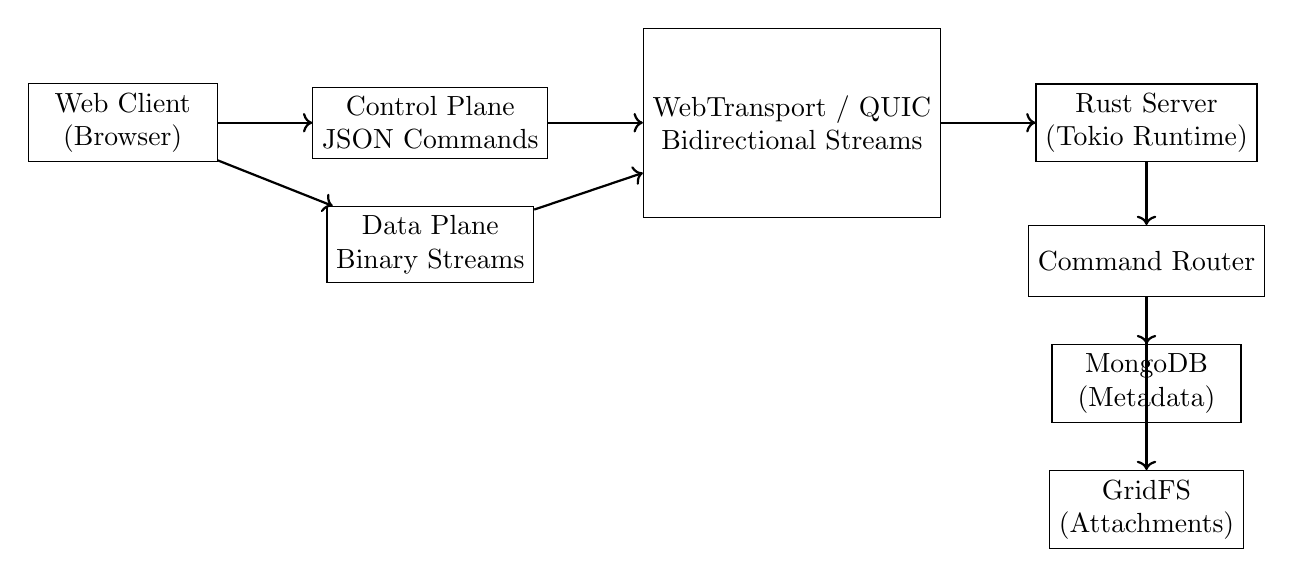
\begin{tikzpicture}[
    box/.style={draw, rectangle, align=center, minimum width=2.4cm, minimum height=0.9cm},
    arrow/.style={->, thick}
]

\node[box] (client) {Web Client\\(Browser)};

\node[box, right=1.2cm of client] (control) {Control Plane\\JSON Commands};
\node[box, below=0.6cm of control] (data) {Data Plane\\Binary Streams};

\node[box, right=1.2cm of control, minimum height=2.4cm] (transport)
{WebTransport / QUIC\\Bidirectional Streams};

\node[box, right=1.2cm of transport] (server)
{Rust Server\\(Tokio Runtime)};

\node[box, below=0.8cm of server] (router) {Command Router};

\node[box, below=0.6cm of router] (mongo) {MongoDB\\(Metadata)};
\node[box, below=0.6cm of mongo] (gridfs) {GridFS\\(Attachments)};

\draw[arrow] (client) -- (control);
\draw[arrow] (client) -- (data);
\draw[arrow] (control) -- (transport);
\draw[arrow] (data) -- (transport);
\draw[arrow] (transport) -- (server);
\draw[arrow] (server) -- (router);
\draw[arrow] (router) -- (mongo);
\draw[arrow] (router) -- (gridfs);

\end{tikzpicture}
\caption{Architectural overview of the WebMail Transport Protocol (WMTP) illustrating the dual-plane design over WebTransport and QUIC.}
\label{fig:wmtp-architecture}
\end{figure}

\subsection{Dual-Plane Protocol Design}

WMTP employs a dual-plane protocol architecture to separate
latency-sensitive control operations from high-throughput data
transfer \cite{quic, webtransport}. This design resolves the
long-standing interference between small control messages
and large attachment transfers observed in legacy email
protocols such as SMTP and IMAP \cite{smtp, imap, base64}.

\subsubsection{Control Plane}

The control plane operates over a single long-lived
bidirectional WebTransport stream \cite{webtransport}.
Protocol commands and responses are encoded as strictly
typed JSON messages, enabling structured parsing and
asynchronous command execution \cite{jmap}. Operations such
as authentication, mailbox navigation, message listing, and
metadata exchange are handled within this plane. By avoiding
ad-hoc text parsing and supporting concurrent in-flight
commands, the control plane achieves low-latency mailbox
interactions without enforcing strict command ordering
\cite{quic, jmap}.

\subsubsection{Data Plane}

The data plane is responsible for transferring message bodies
and attachments. For each attachment transfer, WMTP creates
an ephemeral bidirectional WebTransport stream dedicated
exclusively to binary data transmission \cite{webtransport}.
Payloads are transmitted as raw binary without Base64
encoding, eliminating the associated size expansion and
processing overhead \cite{base64}. Because data plane streams
are isolated at the QUIC transport level, congestion or packet
loss affecting a large file transfer does not impact ongoing
control operations \cite{quic}.

\subsection{State and Session Management}

WMTP leverages QUIC’s connection identification mechanism
to support persistent sessions across network changes
\cite{quic}. Connections are identified using a 64-bit
connection identifier rather than an IP address and port tuple,
enabling native connection migration. As a result, active
sessions can survive transitions between network interfaces,
such as switching from Wi-Fi to cellular networks, without
requiring re-authentication.

To maintain session liveness and prevent network address
translation (NAT) timeouts, the server periodically transmits
lightweight heartbeat messages over the control plane stream
\cite{webtransport}. These heartbeats allow both endpoints to
detect connection failures and maintain long-lived sessions
reliably. Furthermore, WMTP inherits QUIC's congestion control mechanisms (e.g., CUBIC or NewReno), ensuring fair bandwidth sharing with concurrent TCP flows and preventing network starvation, a critical requirement for deployment in shared network environments.

To ensure scalability and protect against resource exhaustion,
WMTP implements a stream-through data handling methodology
that avoids buffering entire attachments in application memory
\cite{gridfs2024}. Incoming binary data is received in chunks over
dedicated attachment streams. Upon receiving metadata
headers, the server identifies the target storage location and
streams the payload directly from the transport buffer into
GridFS \cite{mongodb2024, gridfs2024}.

This pipeline ensures constant memory usage regardless of
attachment size and allows the system to handle large file
transfers efficiently. By avoiding full in-memory buffering,
WMTP reduces susceptibility to denial-of-service attacks based
on oversized payloads and improves overall system stability
\cite{rustasync}.

\vspace{12pt}
\section{Implementation}

The implementation of the WebMail Transport Protocol
(WMTP) translates the proposed dual-plane architecture into
a fully functional system using high-performance systems
programming techniques and browser-native web APIs
\cite{klabnik2019, rustasync, webtransport, quic}.

\subsection{Server-Side Implementation}

The server is implemented in the Rust programming
language \cite{klabnik2019}, selected for its memory safety guarantees,
zero-cost abstractions, and suitability for low-level protocol
development. Concurrency and asynchronous I/O are managed
using the \textit{tokio} runtime \cite{rustasync}, which enables the
server to efficiently handle a large number of concurrent
WebTransport sessions \cite{webtransport}.

Each incoming WebTransport session is managed as a
lightweight asynchronous task, allowing the server to scale
to thousands of concurrent client connections with minimal
context-switching overhead \cite{rustasync}. The transport layer is
implemented using the \textit{wtransport} library, which
provides a high-level interface over the QUIC protocol
\cite{quic}. A single server endpoint listens for incoming
connections, performs TLS~1.3 handshakes \cite{tls13} using
either self-signed or certificate-authority (CA)-signed
certificates, and demultiplexes bidirectional streams into
control and data planes \cite{quic, webtransport}.

Incoming control plane messages are routed through a
centralized command-processing engine that dispatches
JSON-encoded protocol commands to dedicated handlers
\cite{jmap}. The current implementation supports
$57$ distinct protocol commands. For example, message
transmission and retrieval are handled by message-specific
handlers, while session-related commands manage
authentication state and connection metadata
\cite{smtp, imap}.

\subsection{Persistence and Binary Streaming}

The persistence layer is implemented using MongoDB
\cite{mongodb2024} to align with the document-oriented nature of
the protocol. User profiles, mailbox structures, and message
metadata are stored as BSON documents, enabling efficient
indexing and query execution through the MongoDB Rust
driver \cite{klabnik2019, mongodb2024}.

To support large attachment transfers, the server integrates
MongoDB GridFS \cite{gridfs2024} with an asynchronous streaming
pipeline. As binary data arrives on a dedicated attachment
stream, it is written directly into GridFS in fixed-size chunks
of $255~\mathrm{KB}$. This stream-through design ensures that
the server’s memory usage remains constant regardless of
attachment size, enabling stable performance even during
multi-gigabyte transfers \cite{mongodb2024, gridfs2024}.

\subsection{Client-Side Implementation}

The client is implemented as a browser-based application
using native JavaScript and the standardized WebTransport
API \cite{webtransport}. This approach enables direct and
secure communication with the WMTP server without relying
on intermediary HTTP-based services \cite{http3}.

A transport abstraction layer encapsulates the WebTransport
API and manages stream lifecycle operations, connection
establishment, and reliable delivery of JSON-encoded control
messages \cite{webtransport, jmap}. On top of this layer, a
protocol mediator component maintains the client-side state
machine, including session tokens and authentication status
\cite{jmap}. This component exposes an asynchronous,
promise-based interface to the user-interface layer, allowing
client applications to invoke any of the supported WMTP
protocol commands in a structured and non-blocking manner
\cite{quic, webtransport}.
\vspace{12pt}
\section{Evaluation and Results}

The evaluation of the WebMail Transport Protocol (WMTP)
demonstrates that replacing TCP-based mail transport with
QUIC and WebTransport significantly improves latency,
throughput, and connection resilience \cite{quic, webtransport, tls13}.
This section presents both quantitative performance
measurements and qualitative observations obtained from
experimental testing.

\subsection{Performance Benchmarks}

Experiments were conducted using a Rust-based WMTP
server \cite{klabnik2019, rustasync} deployed on a multi-core system and a
Chromium-based client supporting native WebTransport
\cite{webtransport}. Table~\ref{tab:perf} summarizes the key
performance metrics.

\begin{table}[H]
\caption{WMTP Performance Benchmarks}
\centering
\begin{tabular}{|l|c|}
\hline
\textbf{Metric} & \textbf{Measured Value} \\
\hline
Connection Handshake Latency & 20.10 ms (1-RTT) \\
Average Command Latency & 3.86 ms \\
Maximum Sustained Throughput & 8,756 requests/s \\
Parallel Stream Setup Time & 38.60 ms (50 streams) \\
\hline
\end{tabular}
\label{tab:perf}
\end{table}

\begin{itemize}
\item \textit{Connection Establishment:} WMTP achieved an
average handshake latency of 20.10 ms using a 1-RTT QUIC
handshake \cite{quic, tls13}, representing a substantial
reduction compared to traditional TCP+TLS connection
establishment \cite{smtp, tls13}.
\item \textit{Command Latency:} The average response time
for control-plane protocol commands was measured at
3.86 ms under normal load \cite{jmap}.
\item \textit{Scalability:} The server sustained up to
8,756 requests per second over a single persistent connection
without degradation in responsiveness \cite{rustasync}.
\item \textit{Stream Multiplexing:} Fifty parallel
bidirectional data streams were opened, transmitted, and
closed within 38.60 ms, demonstrating efficient stream
lifecycle management \cite{quic, webtransport}.
\end{itemize}

\subsection{Throughput Analysis}

One of the primary objectives of WMTP is eliminating the
Base64 encoding overhead required by legacy email
protocols \cite{base64, smtp, imap}. Throughput measurements
comparing raw binary transmission with Base64-encoded
transfers are shown in Table~\ref{tab:throughput}.

\begin{table}[H]
\caption{Throughput Comparison: Legacy SMTP vs WMTP}
\centering
\begin{tabular}{|c|c|c|c|}
\hline
\textbf{Payload Size} & \textbf{SMTP + Base64} & \textbf{WMTP (Raw Binary)} & \textbf{Improvement} \\
\hline
1 MB  & 10.00 MB/s & 29.41 MB/s & 2.9$\times$ \\
10 MB & 9.00 MB/s  & 33.78 MB/s & 3.7$\times$ \\
\hline
\end{tabular}
\label{tab:throughput}
\end{table}

WMTP consistently outperformed legacy approaches due to
the elimination of payload expansion and reduced CPU
overhead \cite{quic}. Raw binary transmission over QUIC
streams resulted in up to a threefold improvement in
effective throughput for large attachments \cite{gridfs2024}. Crucially, for mobile devices, this reduction in processing translates directly to improved energy efficiency, as the CPU cycles previously wasted on Base64 encoding/decoding are eliminated.

\subsection{Connection Resilience and Stability}

WMTP exhibited strong resilience under adverse network
conditions. Due to QUIC’s stream-level independence
\cite{quic}, packet loss affecting one stream did not impact
concurrent control or data streams, effectively eliminating
concurrent control or data streams, effectively eliminating
application-layer head-of-line blocking \cite{quic, tls13}. From a security perspective, the protocol mitigates UDP amplification attacks by enforcing strict address validation tokens during the handshake, ensuring that unverified clients cannot trigger large server responses.

In addition, active sessions remained intact during network
transitions, such as switching from Wi-Fi to cellular
networks, without requiring reconnection or
re-authentication \cite{quic, webtransport}. This behavior
highlights the advantages of QUIC connection identifiers
over traditional TCP socket bindings \cite{smtp}.

\subsection{Resource Utilization}

During large attachment transfers, server memory usage
remained constant regardless of file size. Binary data was
streamed directly from the network layer into MongoDB
GridFS \cite{mongodb2024, gridfs2024} without full buffering in
application memory, ensuring predictable and stable
resource consumption \cite{klabnik2019, rustasync}.
\vspace{12pt}
\section{Discussion and Limitations}

While WMTP demonstrates significant performance and
resilience improvements over legacy email protocols, several
limitations remain. First, the current implementation relies on
WebTransport support in modern browsers, which may limit
immediate deployment on older client platforms \cite{webtransport}.
Second, WMTP is designed primarily for client-to-server
communication and does not attempt to replace the global
SMTP-based mail relay infrastructure; integration with existing
mail servers via gateways is necessary for interoperability
\cite{smtp, imap}.

Additionally, QUIC traffic may be subject to blocking or rate
limiting by restrictive network middleboxes in certain enterprise
environments \cite{quic}. Although QUIC adoption is
increasing, deployment in highly controlled networks remains
challenging \cite{http3}. Another consideration is that while
WMTP eliminates Base64 overhead for attachments, extremely
high concurrency with multiple large streams may still stress
CPU resources due to encryption overhead and stream
CPU resources due to encryption overhead and stream
scheduling costs \cite{quic, webtransport, tls13}.

\subsection{Interoperability and Transition Strategy}
A major barrier to adoption is the inertia of the existing SMTP ecosystem. WMTP addresses this via a ``Client-to-Edge'' deployment model. In this architecture, mobile and web clients communicate with a WMTP Edge Server via the optimized protocol, while the Edge Server acts as a gateway, translating messages to standard SMTP for inter-domain delivery (e.g., to Gmail or Outlook). This provides the performance benefits of WMTP to the end-user (the "last mile") without requiring global infrastructure upgrades.

WMTP also currently lacks advanced server-side features
commonly found in enterprise email systems, such as detailed
access control policies, spam filtering, and message auditing,
which are necessary for production deployments \cite{smtp, jmap}.
Furthermore, the dual-plane architecture introduces additional
protocol complexity that requires careful stream lifecycle
management. Unlike stateless HTTP/REST architectures, WMTP's stateful nature requires the server to maintain session contexts. While this theoretically limits horizontal scalability compared to stateless web services, our benchmarks indicate that the reduction in handshake overhead and connection re-establishment costs outweighs the memory cost of maintaining state for typical email usage patterns.

Finally, although WMTP leverages MongoDB GridFS for
efficient large-object storage, persistence performance may
vary under extremely high load or adverse network conditions,
highlighting the need for optimized database replication and
sharding strategies \cite{mongodb2024, gridfs2024}. Future work will
explore adaptive stream prioritization, intelligent congestion
management, and fallback mechanisms to HTTP/2 or
WebSocket-based transports for environments where
WebTransport or QUIC is unavailable \cite{http3, jmap}.
\vspace{12pt}
\section{Conclusion and Future Work}

This work introduced the WebMail Transport Protocol (WMTP), a modern mail transport protocol designed around WebTransport and the QUIC transport layer \cite{smtp,quic}. Unlike legacy email protocols that rely on sequential, TCP-based communication models \cite{smtp,imap}, WMTP adopts a stream-oriented and multiplexed design aligned with the requirements of contemporary web and mobile applications. By exposing QUIC’s bidirectional streams directly to the application layer, WMTP enables low-latency interactions, efficient binary data transfer, and resilient long-lived sessions within a single encrypted connection \cite{tls13,quic}.

A key contribution of this work is the dual-plane protocol architecture, which separates control signaling from bulk data transfer \cite{jmap,webtransport}. This separation allows latency-sensitive operations such as authentication, mailbox navigation, and message metadata retrieval to proceed independently of large attachment transfers \cite{smtp,imap,base64}. Experimental evaluation shows that this design effectively eliminates application-layer head-of-line blocking and enables predictable performance under concurrent workloads \cite{quic,webtransport}. Moreover, the use of raw binary streams avoids Base64 encoding overhead, resulting in improved throughput and reduced CPU utilization \cite{base64,gridfs2024}.

The feasibility of WMTP was validated through a complete end-to-end implementation comprising a Rust-based asynchronous server \cite{rustasync,klabnik2019} and a browser-native WebTransport client \cite{webtransport}. The server architecture leverages non-blocking I/O and streaming mechanisms to maintain bounded memory usage regardless of attachment size \cite{mongodb2024,gridfs2024}. Experimental results indicate that WMTP achieves lower connection establishment latency, higher sustained throughput, and seamless connection migration when compared with traditional SMTP- and IMAP-based workflows \cite{smtp,imap,quic}.

Beyond performance gains, WMTP demonstrates the broader applicability of WebTransport as a foundation for application-layer protocols traditionally constrained by TCP semantics \cite{http3,webtransport}. By integrating transport-level multiplexing, encryption, and connection migration into the protocol design, WMTP illustrates how legacy communication systems can be re-engineered for web-native environments without compromising reliability or security \cite{tls13,quic}.

Future work will focus on extending WMTP toward production-ready deployment. Planned enhancements include interoperability gateways that integrate WMTP with existing SMTP-based mail infrastructure, enabling incremental adoption without disrupting global email delivery \cite{smtp,imap}. Further research will investigate advanced security mechanisms such as fine-grained access control, message integrity auditing, and abuse prevention \cite{tls13,jmap}. Finally, large-scale evaluations under heterogeneous mobile network conditions and multi-tenant server deployments will be conducted to further assess WMTP’s scalability and real-world performance \cite{quic,webtransport,rustasync}.

\footnotesize
\begin{thebibliography}{15}

\bibitem{smtp}
Klensin, J.: Simple Mail Transfer Protocol. RFC 5321 (2008)

\bibitem{imap}
Crispin, M.: Internet Message Access Protocol—Version 4rev1. RFC 3501 (2003)

\bibitem{base64}
Freed, N., Borenstein, N.: Multipurpose Internet Mail Extensions (MIME) part one. RFC 2045 (1996)

\bibitem{jmap}
Newman, C., Melnikov, S.: The JSON Meta Application Protocol (JMAP). RFC 8620 (2019)

\bibitem{quic}
Iyengar, J., Thomson, M.: QUIC: A UDP-based multiplexed and secure transport. RFC 9000 (2021)

\bibitem{tls13}
Rescorla, E.: The Transport Layer Security (TLS) protocol version 1.3. RFC 8446 (2018)

\bibitem{http3}
Bishop, M.: HTTP/3. RFC 9114 (2022)

\bibitem{webtransport}
W3C: WebTransport. W3C Recommendation (2023)

\bibitem{rustasync}
Tokio Contributors: Tokio: An asynchronous runtime for Rust (2024). \url{https://tokio.rs}

\bibitem{klabnik2019}
Klabnik, S., Nichols, C.: The Rust Programming Language. No Starch Press, San Francisco (2019)

\bibitem{mongodb2024}
MongoDB Inc.: MongoDB documentation (2024). \url{https://www.mongodb.com/docs}

\bibitem{gridfs2024}
MongoDB Inc.: GridFS specification (2024). \url{https://www.mongodb.com/docs/manual/core/gridfs}

\end{thebibliography}

\end{document}
